% variables of line 
% 	beginning (two numbers), 
% 	direction 
%		0 - left, 
%       1 left-up, 
%       2 up, 
%       3 right-up, 
%       4 right
%	special point (two numbers)
% 	move number (one number)
% together 6 variables 


\newcounter{curx}
\newcounter{cury}

\newcommand{\unitsize}{0.5cm}
\newcommand{\unitscale}{0.5}

\newcommand*{\linemorpion}[6]{
    \setcounter{curx}{#1}
    \setcounter{cury}{#2}
    \foreach \vertex in {0,...,3}
	{
    	\ifthenelse{\vertex = #5} 
        {
        	\node (current) [draw,circle] at (\value{curx}*\unitscale,\value{cury}*\unitscale) {#6};
        }
        {
        	\node (current) [draw=none] at (\value{curx}*\unitscale,\value{cury}*\unitscale) {};
        }
        \node (new)  at ((\value{curx}*\unitscale+#3*\unitscale,\value{cury}*\unitscale+#4*\unitscale) {};
        \path (current) edge (new); 
        \setcounter{curx}{\value{curx}+#3};
        \setcounter{cury}{\value{cury}+#4};
	}
}

\newcommand*\morpion{
\node(place) at (0,0)  {};
\foreach \edge in {0,...,11}
{ 			
		\ifthenelse{\equal{\intcalcMod{\edge}{2}}{0}} 
        	{ 
				\ifthenelse{\edge < 6}{ 
					\foreach \i in {1,2,3} 
					{
						\node[above of=place] (place) {};
					}
				}
				{	
					\foreach \i in {1,2,3} 
					{
						\node[below of=place] (place) {};
					}
				}
			}
			{
				\ifthenelse{\edge < 8 \AND \edge > 2}
                {
					\foreach \i in {1,2,3}
					{
					\node[right of=place] (place) {};
					}
				}
				{	
					\foreach \i in {1,2,3} 
					{
						\node[left of=place] (place) {};
					}
				}
			}
}
}

\begin{figure}
\begin{center}
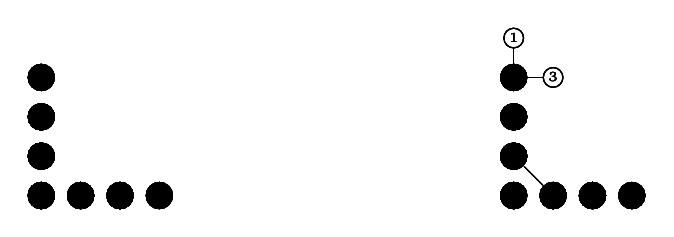
\begin{tikzpicture}%[scale=0.3]
\tikzstyle{every node}=[draw,%
			circle,%
			fill,%
			minimum size  = 0.5*\unitsize,%
			node distance = \unitsize] 
\morpion
\begin{scope}[shift={(6,0)}]
\morpion
\end{scope}
\begin{scope}[shift={(6,0)}]
\tikzstyle{every node}=[minimum size  = 0.5*\unitsize,%
			node distance = unitsize,{font=\tiny},inner sep=0pt] 
\linemorpion{0}{4}{0}{-1}{0}{1}
\linemorpion{1}{0}{-1}{1}{2}{2}
\linemorpion{1}{3}{-1}{0}{0}{3}
\end{scope}
\end{tikzpicture}
\caption{Initial position of Morption 5T on the left and a position with 3 moves on the right.}
\label{fig:rules}
\end{center}
\end{figure}


